\subsection{Disposición en bloques y mapeo del vector de estado}

La primera parte del desarrollo consistió en introducir una disposición explícita del vector de estado en bloques contiguos. Cada bloque agrupa una
cantidad fija de estados base y almacena sus componentes real e imaginaria en forma intercalada. Con ello, cualquier estado base puede mapearse a un
índice de bloque y a un desplazamiento local dentro de ese bloque.

Esta capa de mapeo es necesaria para que el esquema identifique rápidamente qué bloque debe adquirirse ante una operación de lectura, escritura o
aplicación de compuerta. También permite tratar el último bloque de manera especial cuando el número total de estados no llena exactamente una unidad
completa de almacenamiento. Esta organización es la base que permite compartir una misma lógica de actualización para representaciones comprimidas y no comprimidas, variando únicamente la materialización física del bloque activo.

\begin{figure}[H]
    \centering
    \caption{Mapeo lógico del vector de estado}
    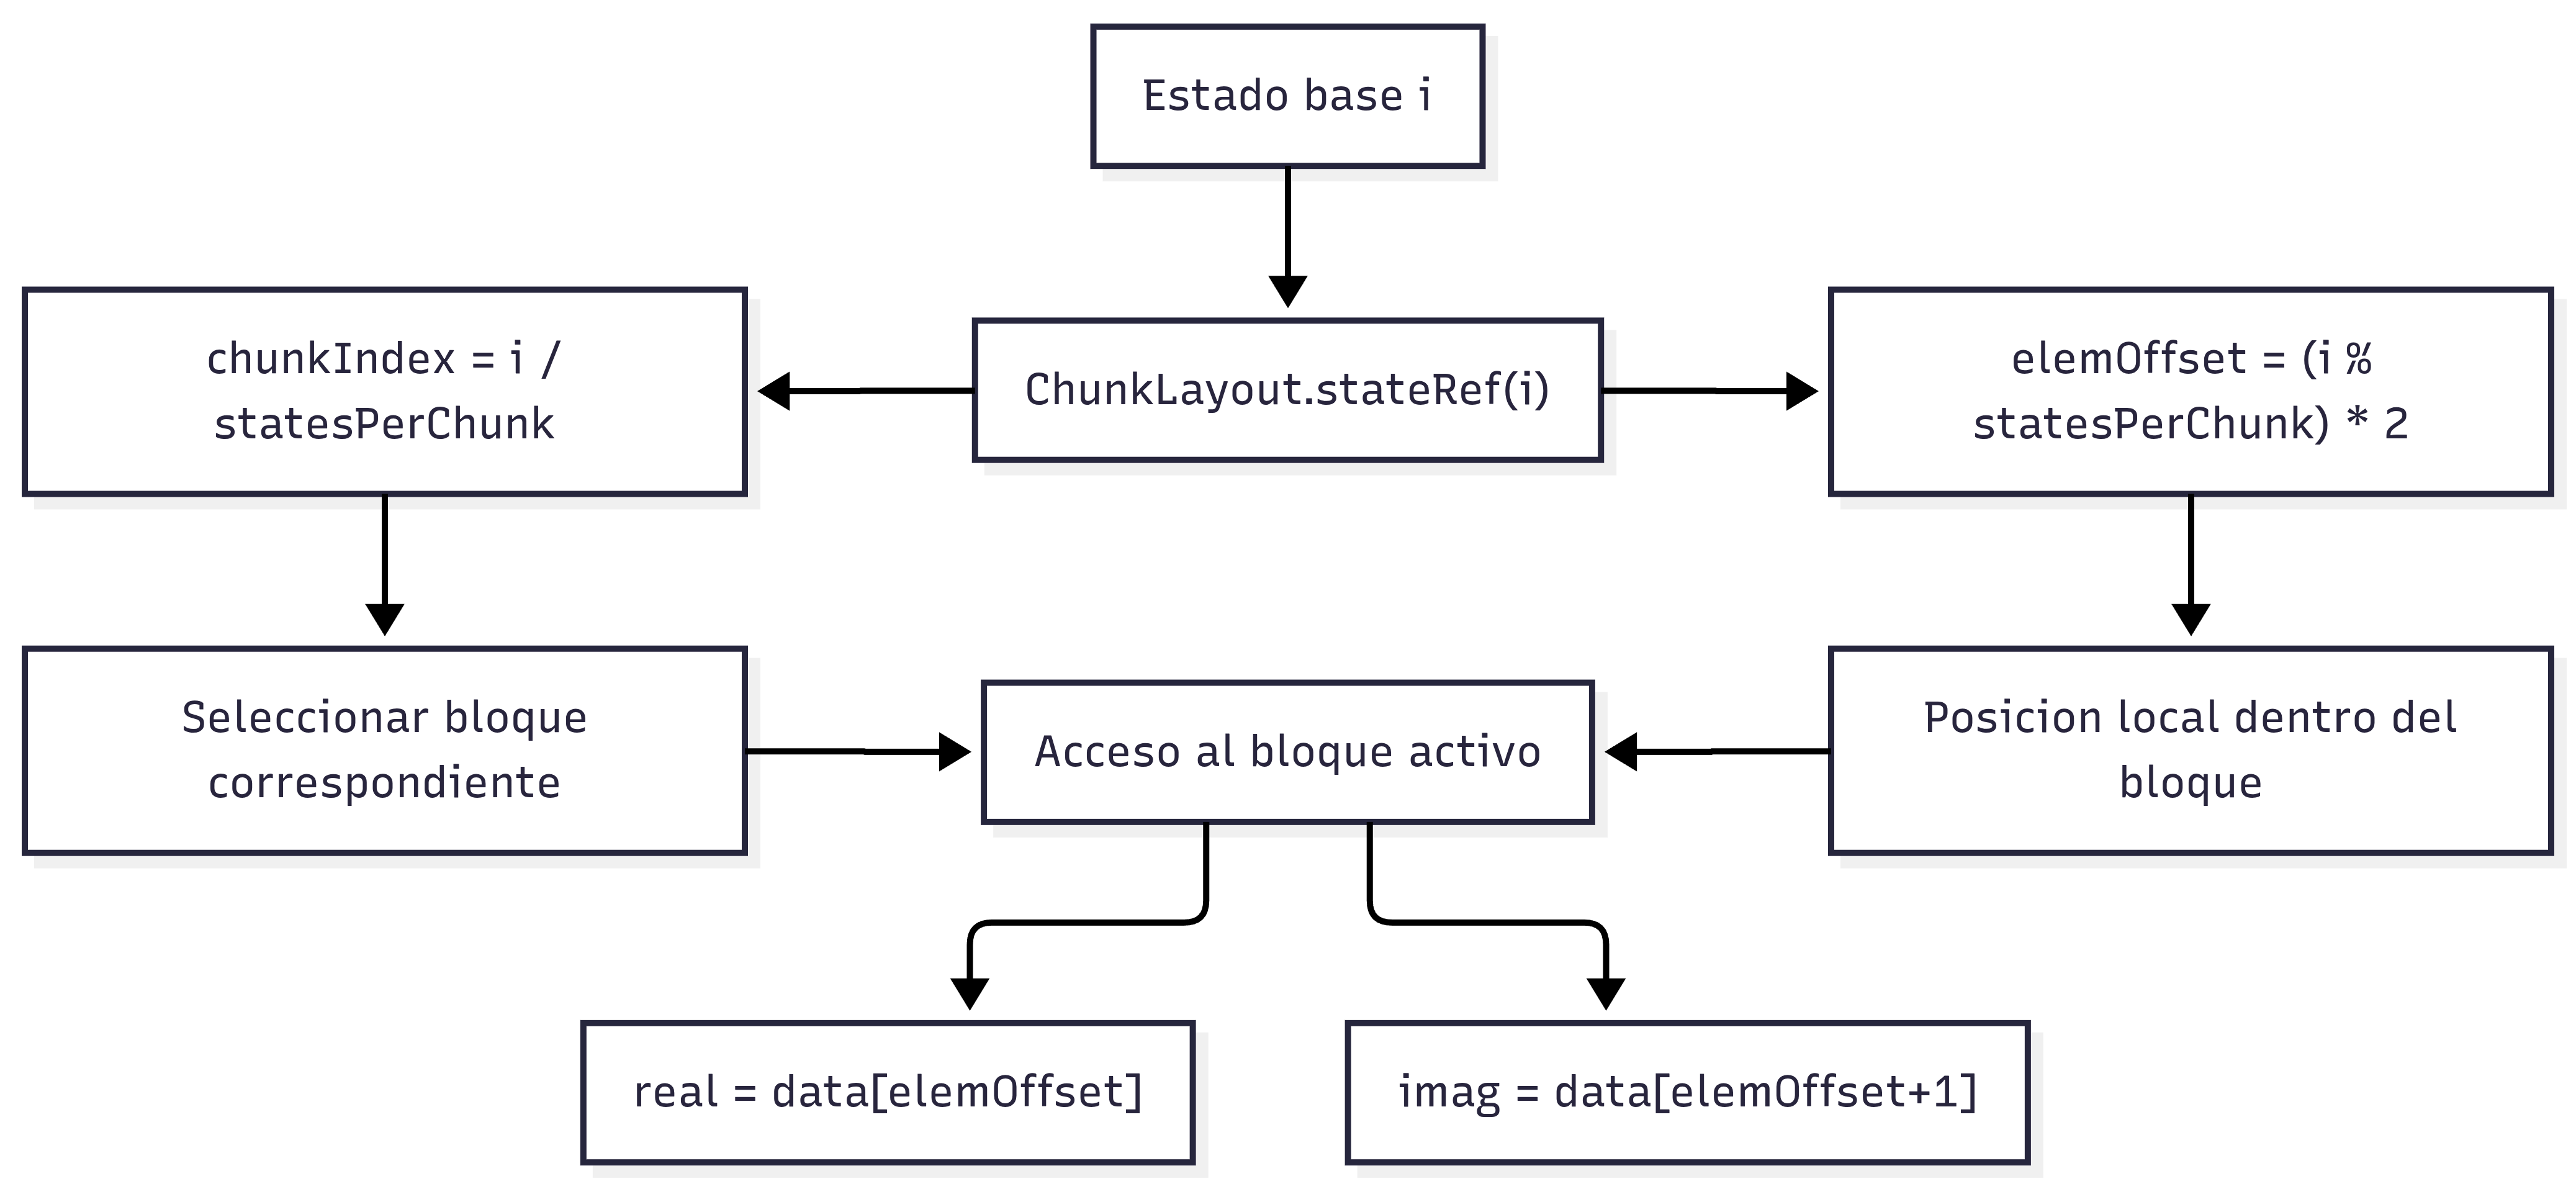
\includegraphics[width=0.8\textwidth]{images/state-vector-chunk-disposition-a.png}
    \label{fig:development-layout-a}
\end{figure}

\begin{figure}[H]
    \centering
    \caption{Acceso al vector de estado según backend}
    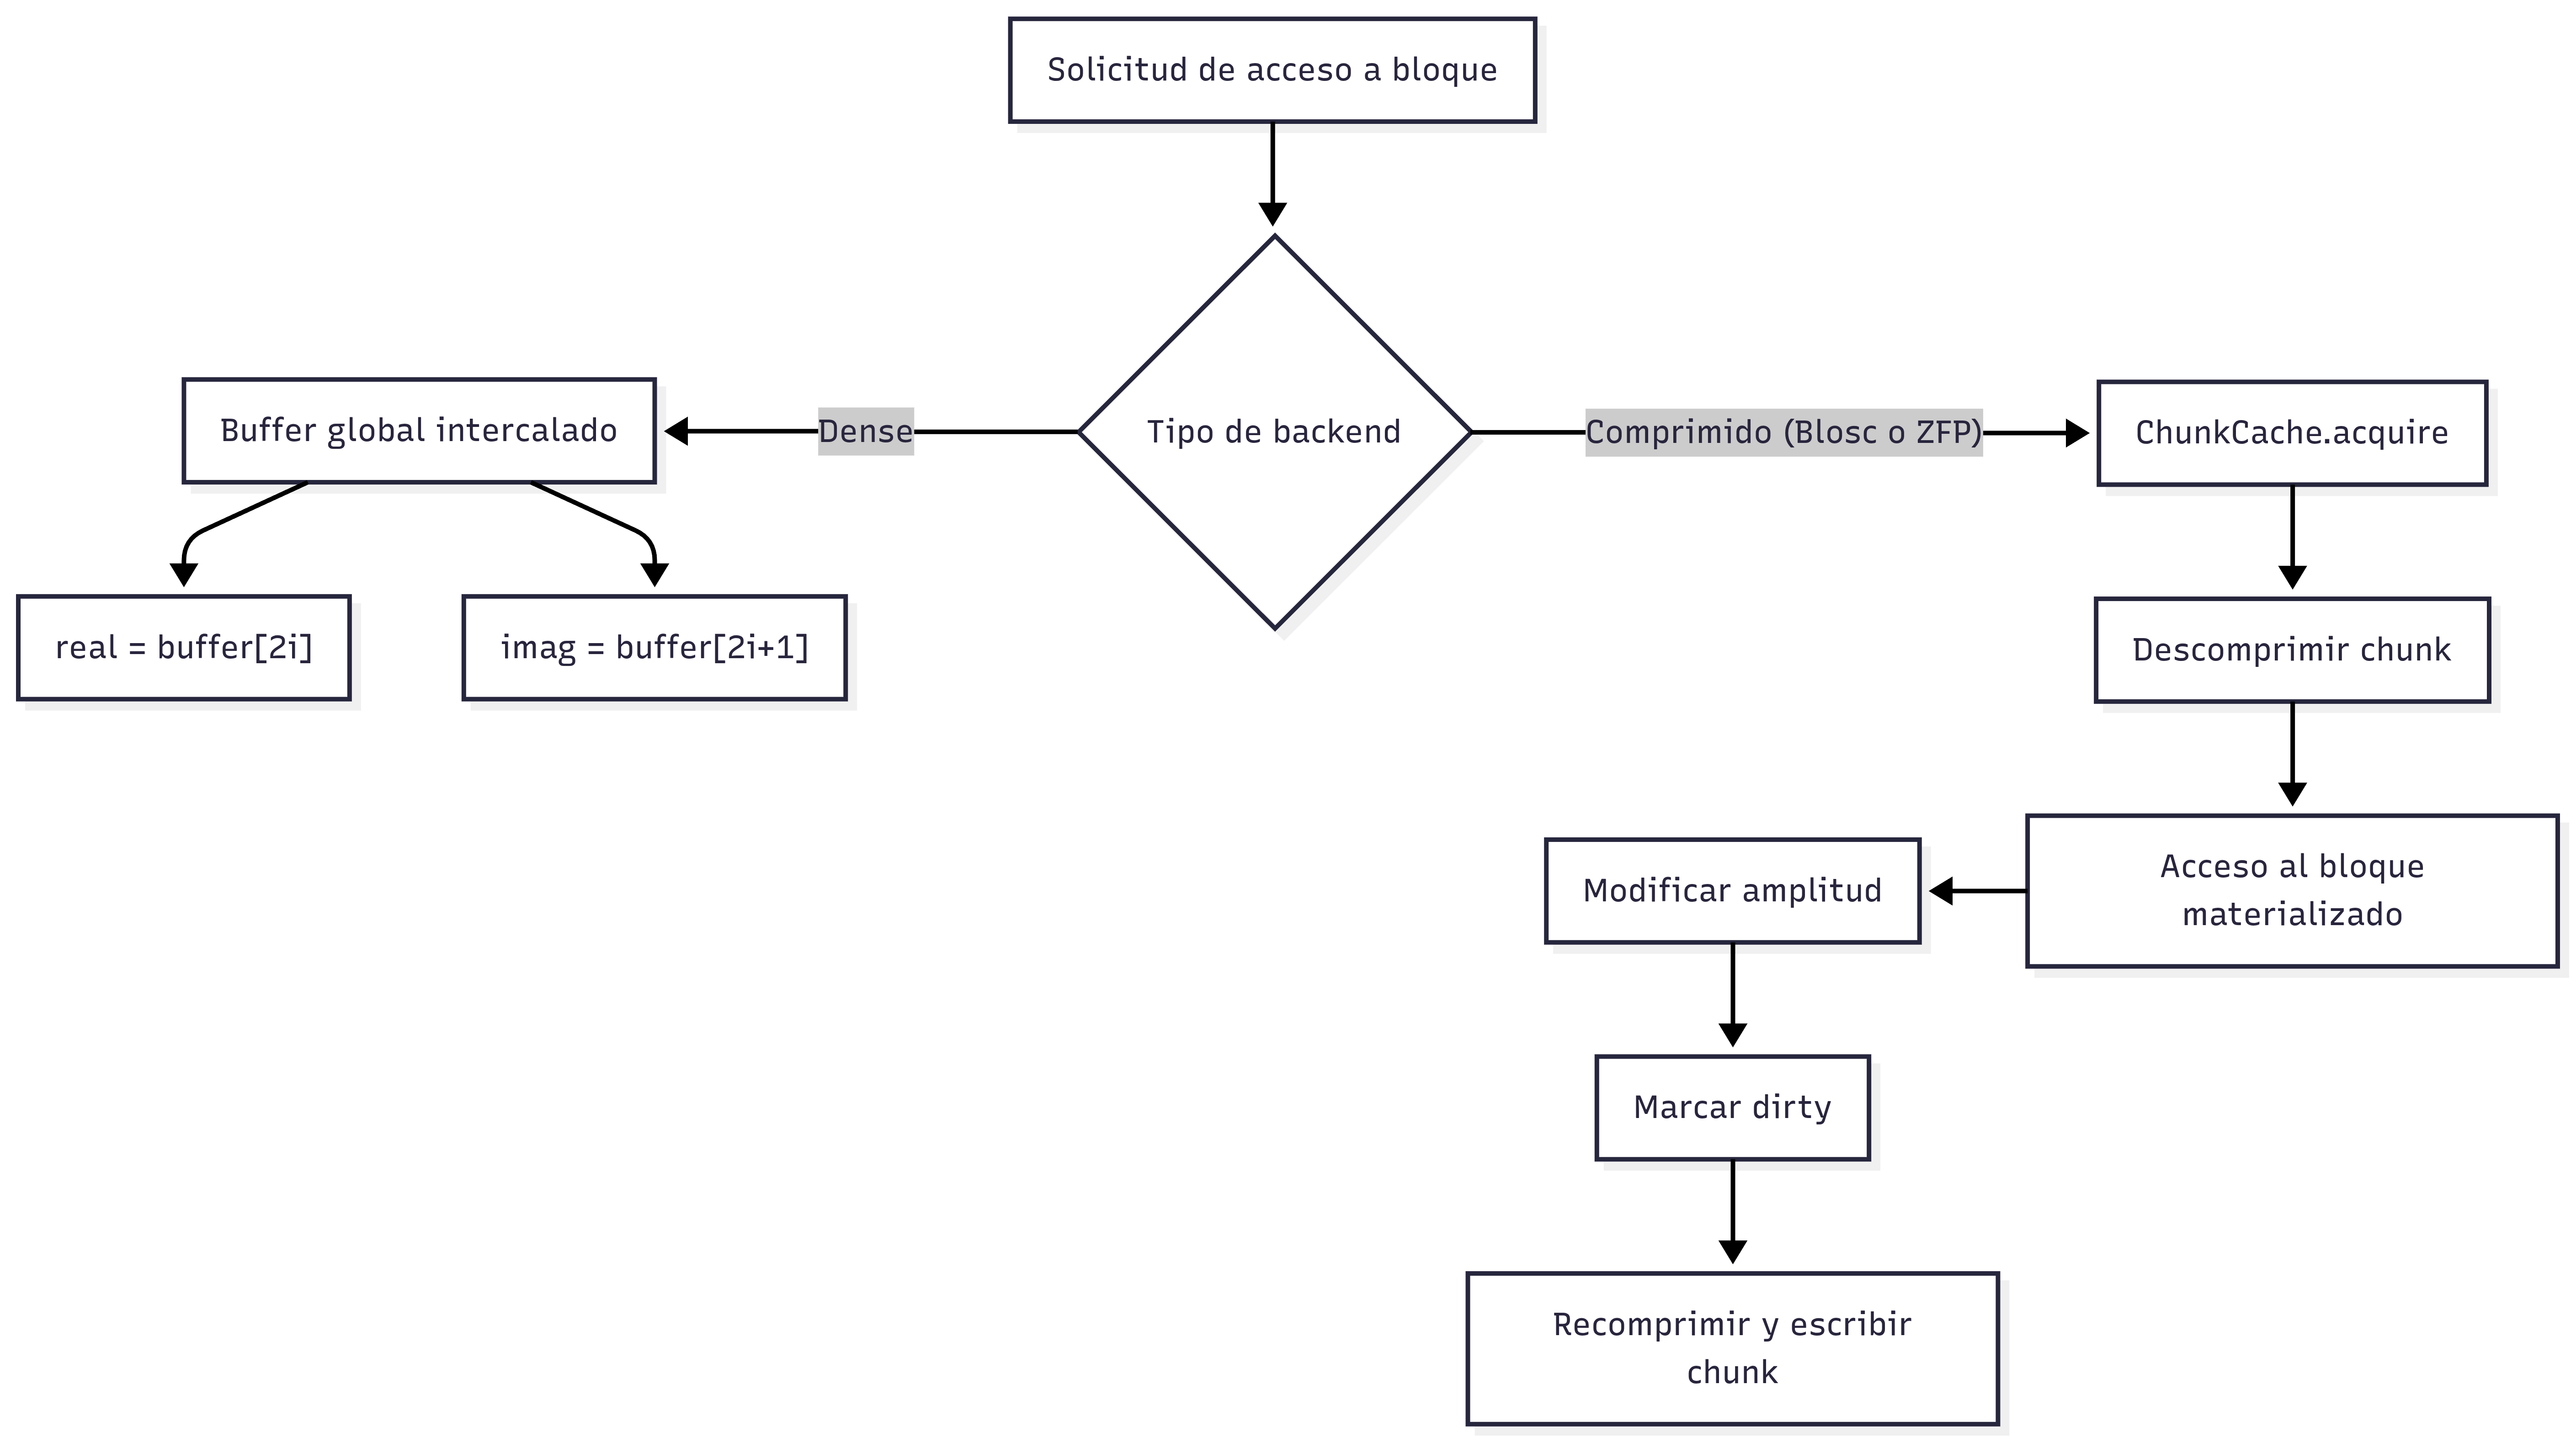
\includegraphics[width=1\textwidth]{images/state-vector-chunk-disposition-b.png}
    \label{fig:development-layout-b}
\end{figure}

\begin{figure}[H]
    \centering
    \caption{Aplicación de compuertas por bloques}
    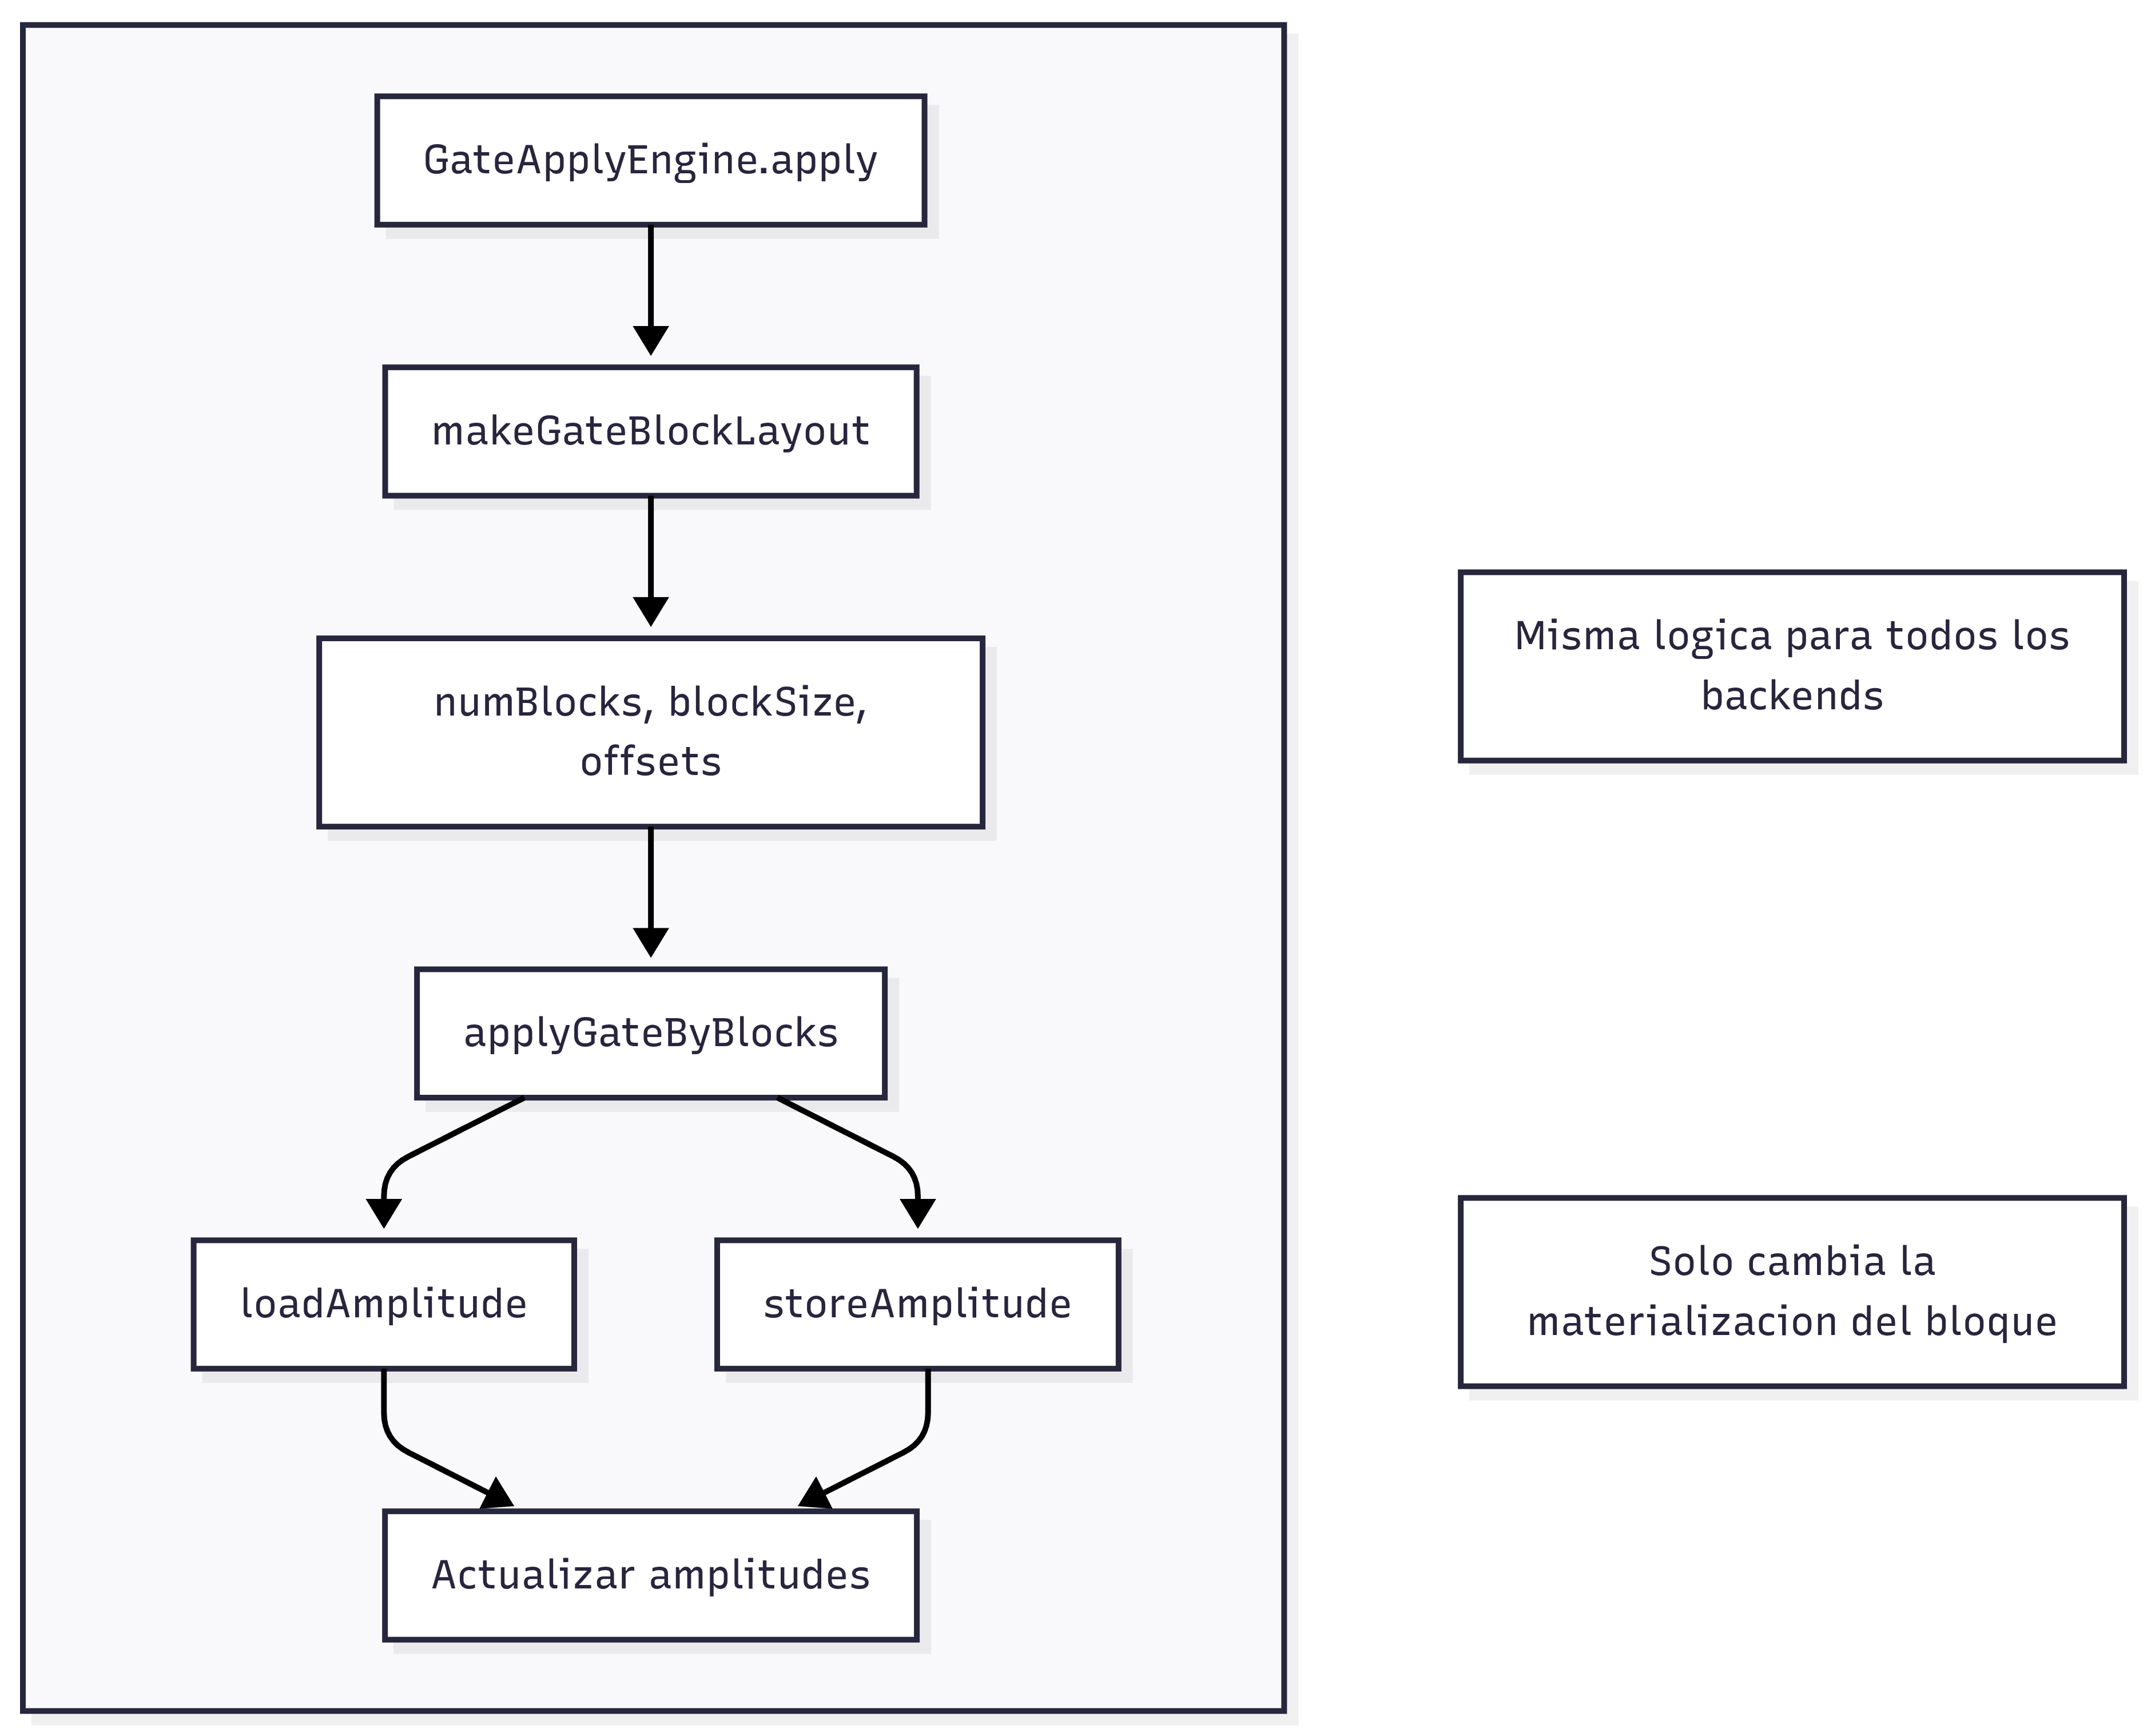
\includegraphics[width=0.7\textwidth]{images/state-vector-chunk-disposition-c.png}
    \label{fig:development-layout-c}
\end{figure}
